\documentclass[%
 reprint,
%superscriptaddress,
%groupedaddress,
%unsortedaddress,
%runinaddress,
%frontmatterverbose, 
%preprint,
%showpacs,preprintnumbers,
%nofootinbib,
%nobibnotes,
%bibnotes,
 amsmath,amssymb,
 aps,
%pra,
%prb,
%rmp,
%prstab,
%prstper,
%floatfix,
]{revtex4-1}

\usepackage{graphicx}% Include figure files
\usepackage{dcolumn}% Align table columns on decimal point
\usepackage{bm}% bold math
%\usepackage{hyperref}% add hypertext capabilities
%\usepackage[mathlines]{lineno}% Enable numbering of text and display math
%\linenumbers\relax % Commence numbering lines

%\usepackage[showframe,%Uncomment any one of the following lines to test 
%%scale=0.7, marginratio={1:1, 2:3}, ignoreall,% default settings
%%text={7in,10in},centering,
%%margin=1.5in,
%%total={6.5in,8.75in}, top=1.2in, left=0.9in, includefoot,
%%height=10in,a5paper,hmargin={3cm,0.8in},
%]{geometry}

\usepackage{cmap} % Поиск в PDF
\usepackage[T2A]{fontenc} % Кодировка
\usepackage[utf8]{inputenc} % Кодировка исходного текста
\usepackage[english, russian]{babel} % Локализация и переносы
\frenchspacing % Более тонкая настройка пробелов 
\usepackage{multirow}
\usepackage[warn]{mathtext}
\usepackage{amssymb}
\usepackage{ dsfont }
\usepackage{ textcomp }
\usepackage{ mathrsfs }

% Переопределение англоязычного начертания каппа, фи и эпсилон, 
% а также знаков сравнения
\renewcommand{\epsilon}{\ensuremath{\varepsilon}}
\renewcommand{\phi}{\ensuremath{\varphi}} 
\renewcommand{\kappa}{\ensuremath{\varkappa}}
\renewcommand{\le}{\ensuremath{\leslant}}
\renewcommand{\leq}{\ensuremath{\leqslant}}
\renewcommand{\ge}{\ensuremath{\geslant}}
\renewcommand{\geq}{\ensuremath{\geqslant}}
\renewcommand{\emptyset}{\ensuremath{\varnothing}}

\usepackage{textcomp} 
\usepackage{indentfirst} % Красная строка
\usepackage{amsmath} % Текст в формулах
\usepackage{graphicx} % Графика
\DeclareGraphicsExtensions{.pdf,.png,.jpg}
\usepackage{pgfplots}
\pgfplotsset{compat=1.13}

%\usepackage{times}

\begin{document}

\title{Экспериментальная проверка уравнения Эйнштейна для фотоэекта}
\thanks{1.1}

\author{Иван Едигарьев}
\affiliation{
 Московский Физико-Технический Институт\\
 Факультет Общей и Прикладной Физики, 526т\\
}
%\date{\today}

\begin{abstract}
В работе исследуется зависимость фототока от величины задерживающего потенциала и частоты падающего излучения, что позволяет вычислить величину постоянной Планка.

\end{abstract}

\pacs{Valid PACS appear here}

\maketitle

\begin{enumerate}

\item 
\textbf{Градуировка монохроматора}\\
Используя окуляр, проградуируем барабан монохроматора по спектру неоновой лампы. Построим градуировочную кривую монохроматора.
\begin{figure}[h]
\center{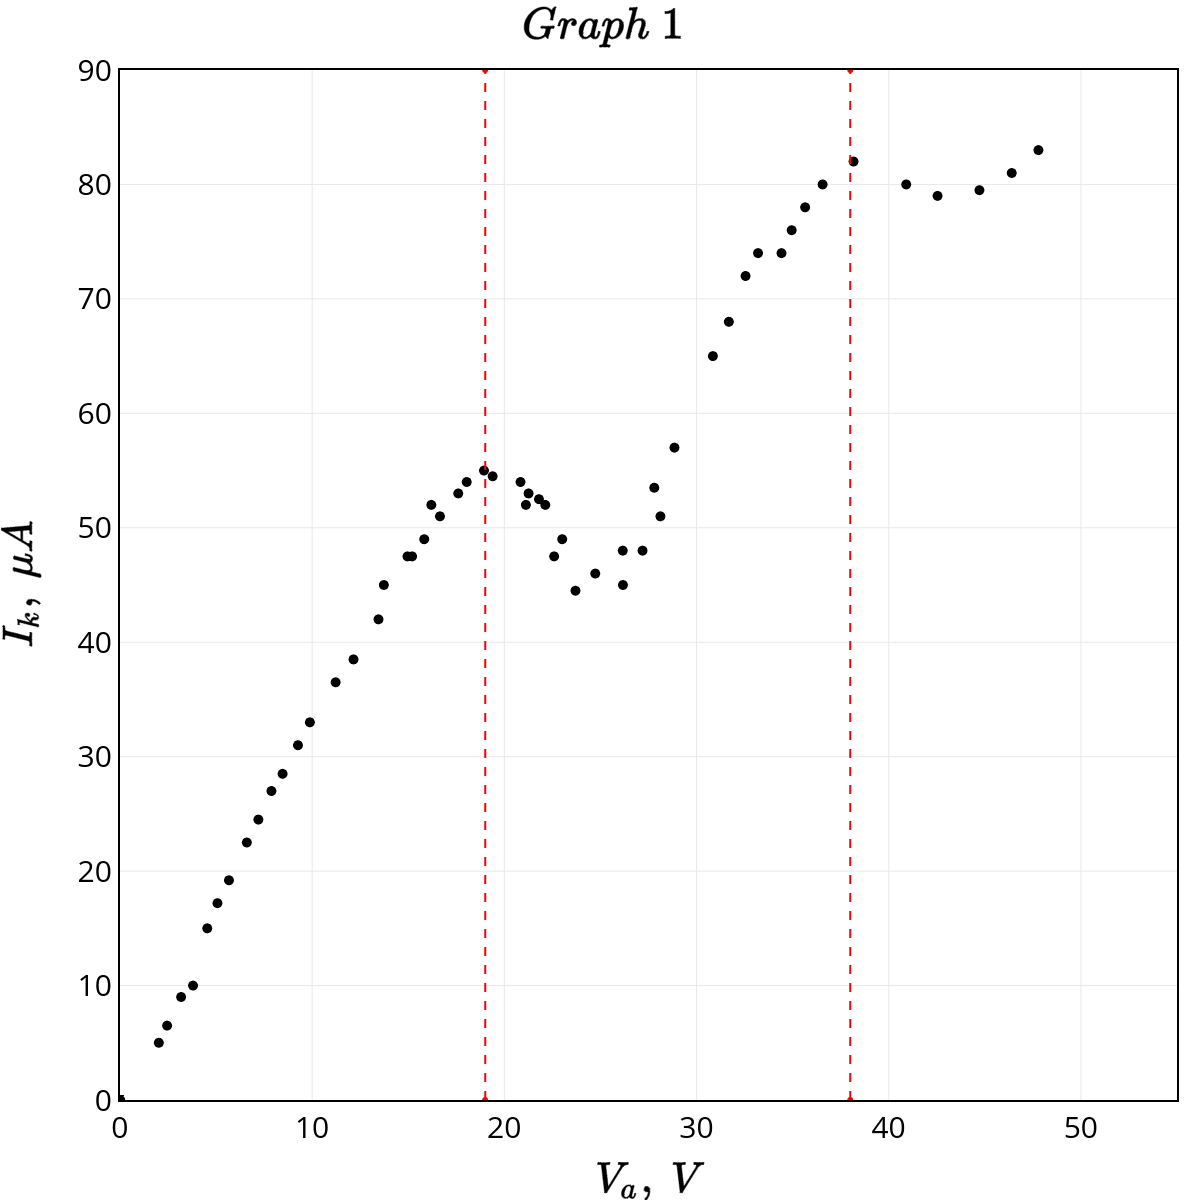
\includegraphics[scale=0.18]{my_plot1.png}}
\end{figure}
\item
\textbf{Исследование зависимости фототока от величины запирающего потенциала}\\
На одном листе построим серию графиков $\sqrt{I} = f(V)$; для каждой длины волны определим величину запирающего потенциала, экстраполируя полученные кривые к оси абсцисс.
\begin{figure}[h]
\center{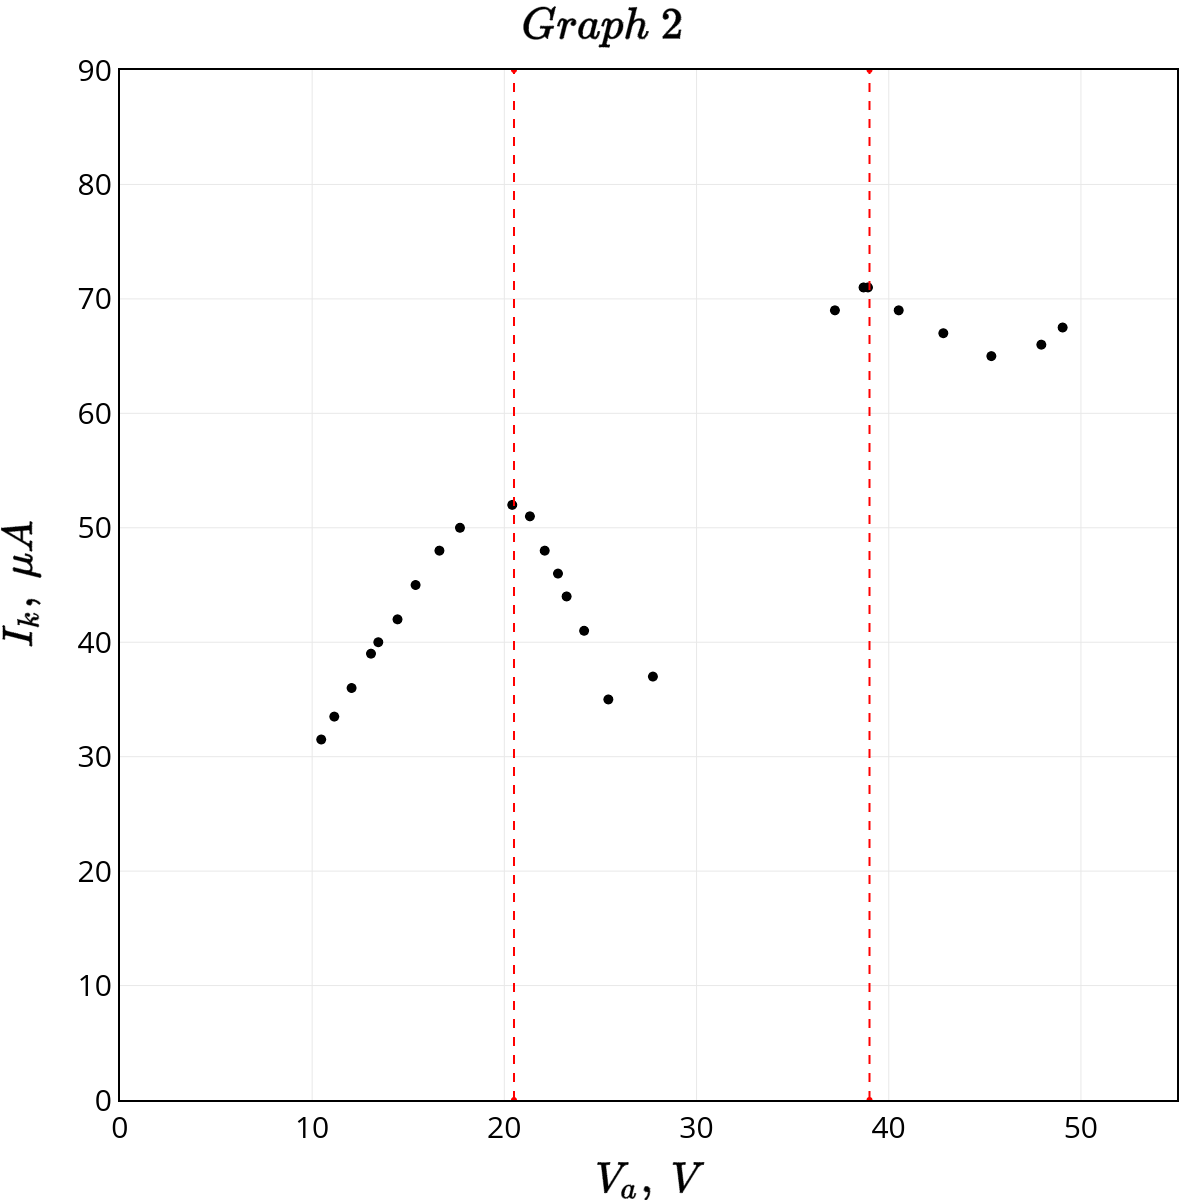
\includegraphics[scale=0.18]{my_plot2.png}}
\end{figure}
Постройте график зависимости $V_0(\omega)$. По графику определим постоянную Планка, оценим погрешность результата и сравним найденное значение с табличным. 
\begin{figure}[h]
\center{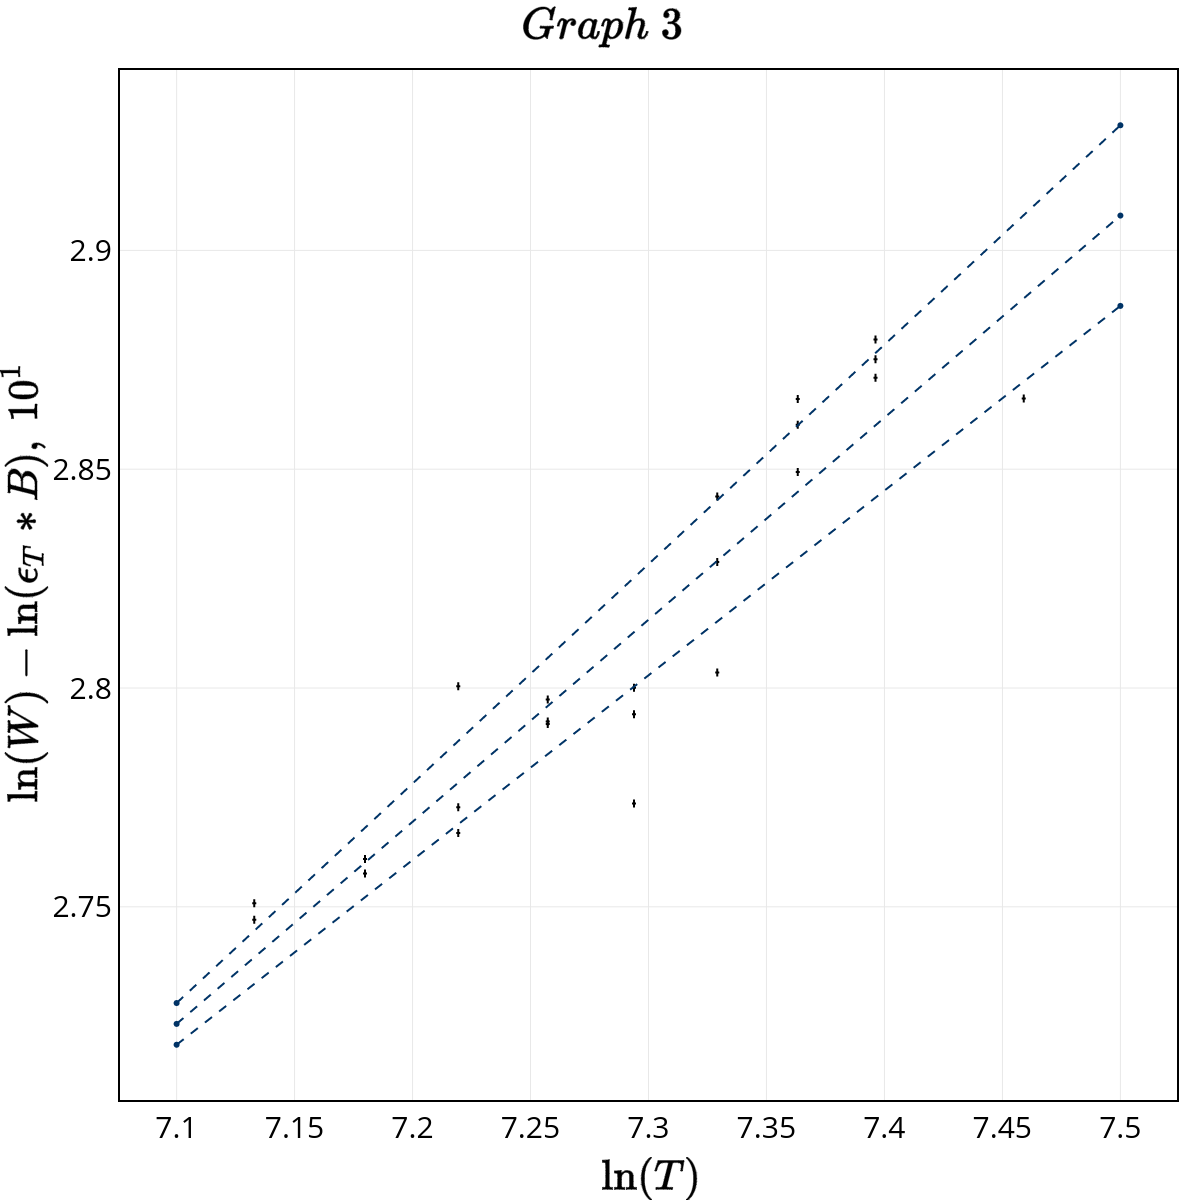
\includegraphics[scale=0.18]{my_plot3.png}}
\end{figure}
\begin{gather*}
b = \frac{dV_0}{d\omega} = (5.9 \pm 0.7)~10^{-16}~V \cdot s,\\
\hbar = (0.9 \pm 0.1)~10^{-34}~J \cdot s,\\
\hbar = 1.054 ~10^{-34}~J \cdot s.
\end{gather*}
Оценим по графику красную границу в ангстремах и работу выхода материала катода в электронвольтах (с точностью до контактной разницы потенциалов).
\begin{gather*}
\lambda_{\text{красн}} = 150~nm,\\
W = 1.1~\text{eV}.
\end{gather*}

\clearpage


\begin{figure}
\center{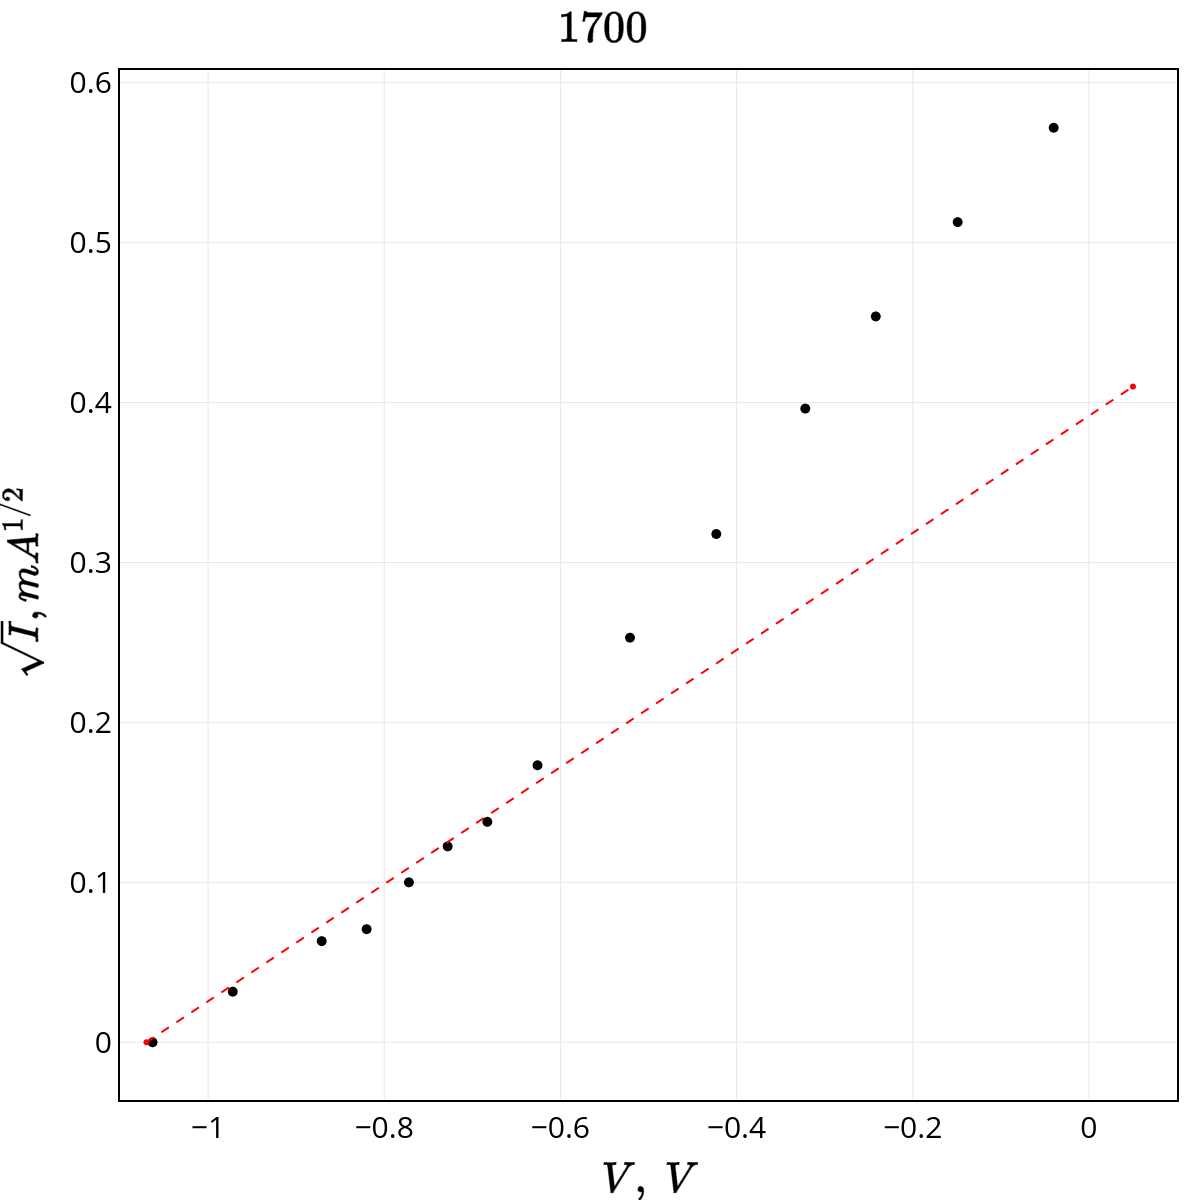
\includegraphics[scale=0.16]{1700.png}}
\center{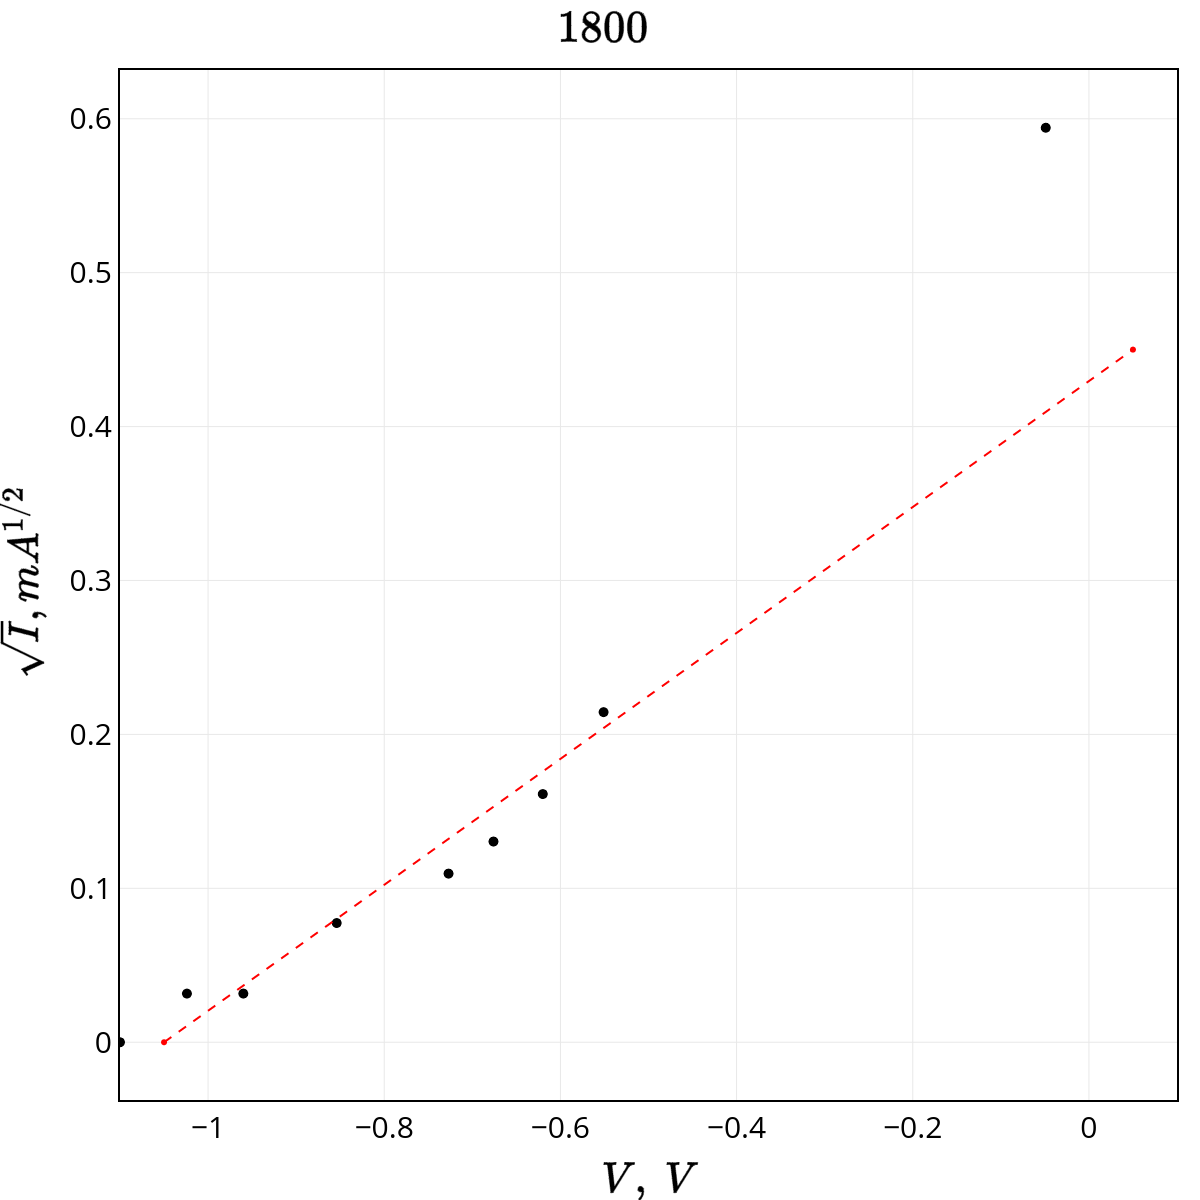
\includegraphics[scale=0.16]{1800.png}}
\center{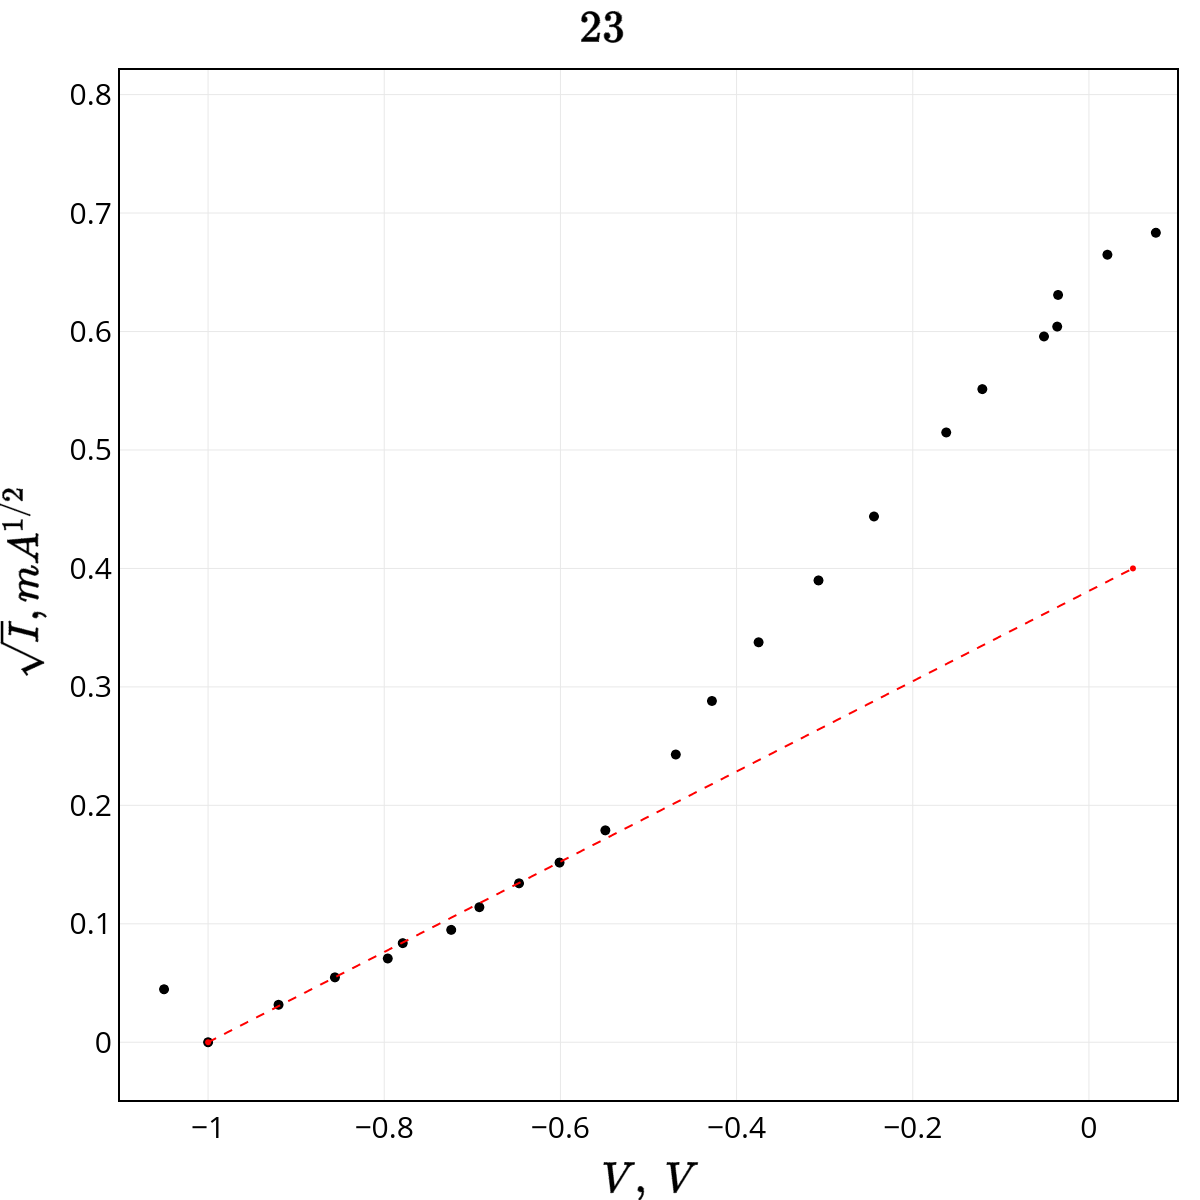
\includegraphics[scale=0.16]{23.png}}
\end{figure}
\begin{figure}
\center{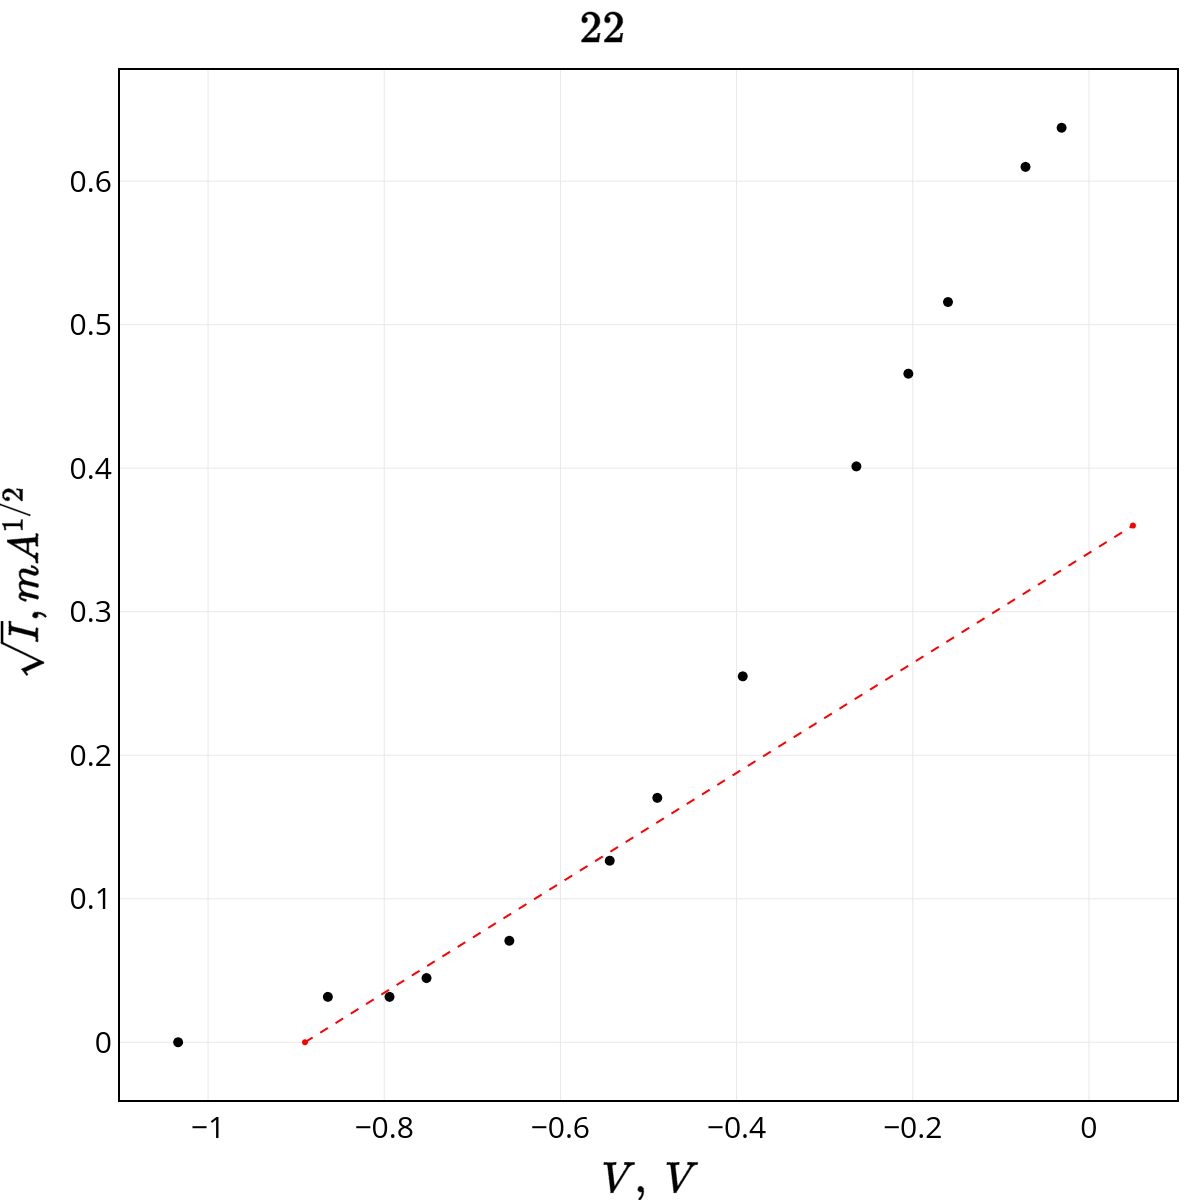
\includegraphics[scale=0.16]{22.png}}
\center{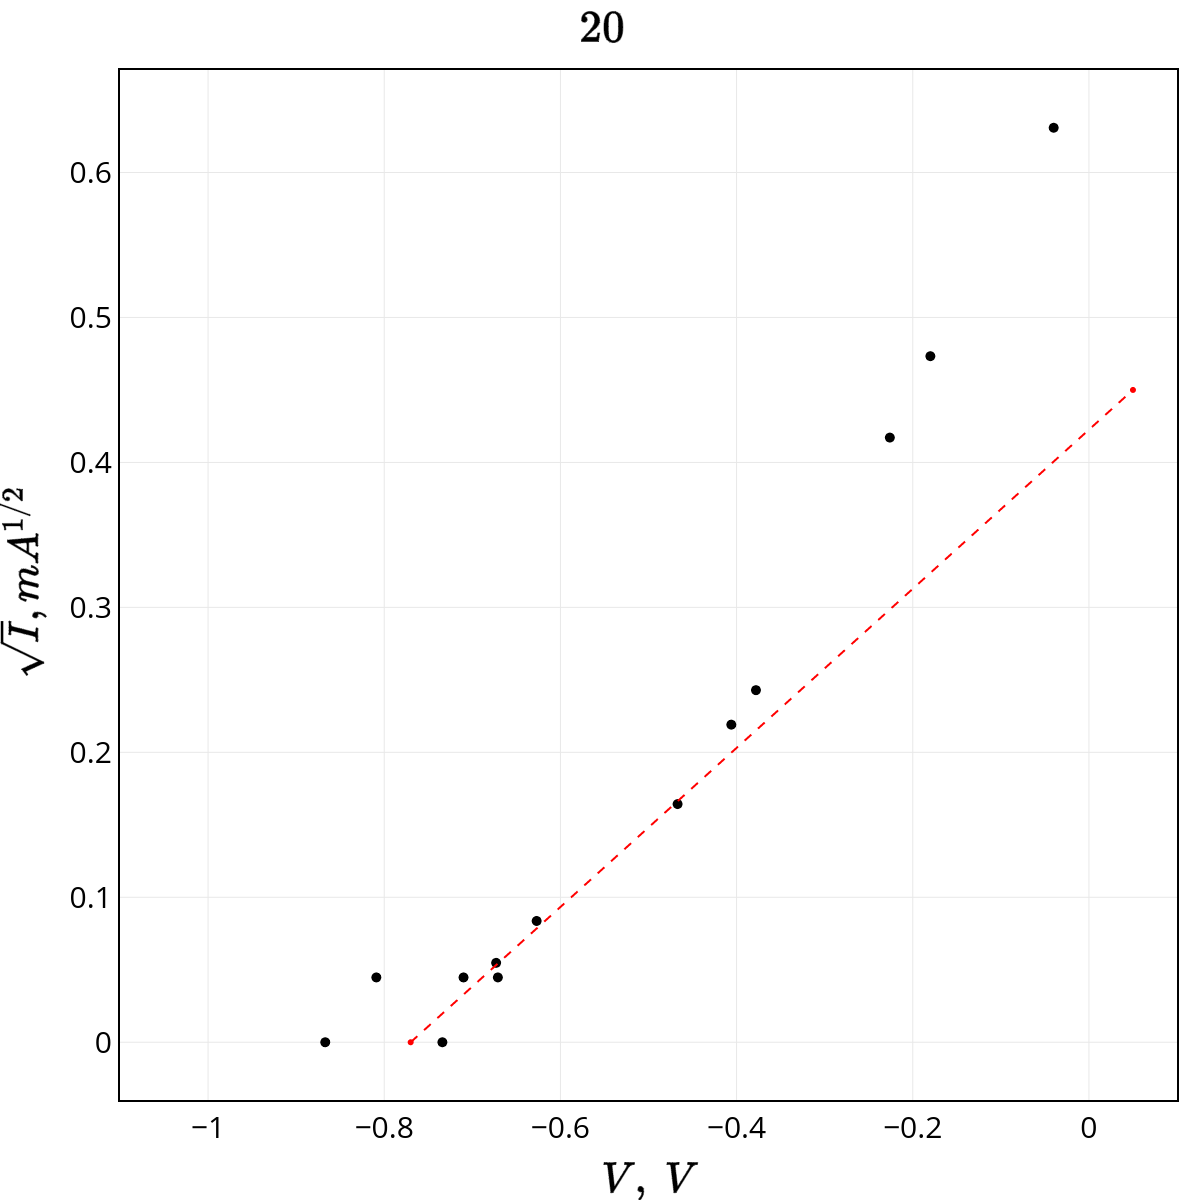
\includegraphics[scale=0.16]{20.png}}
\center{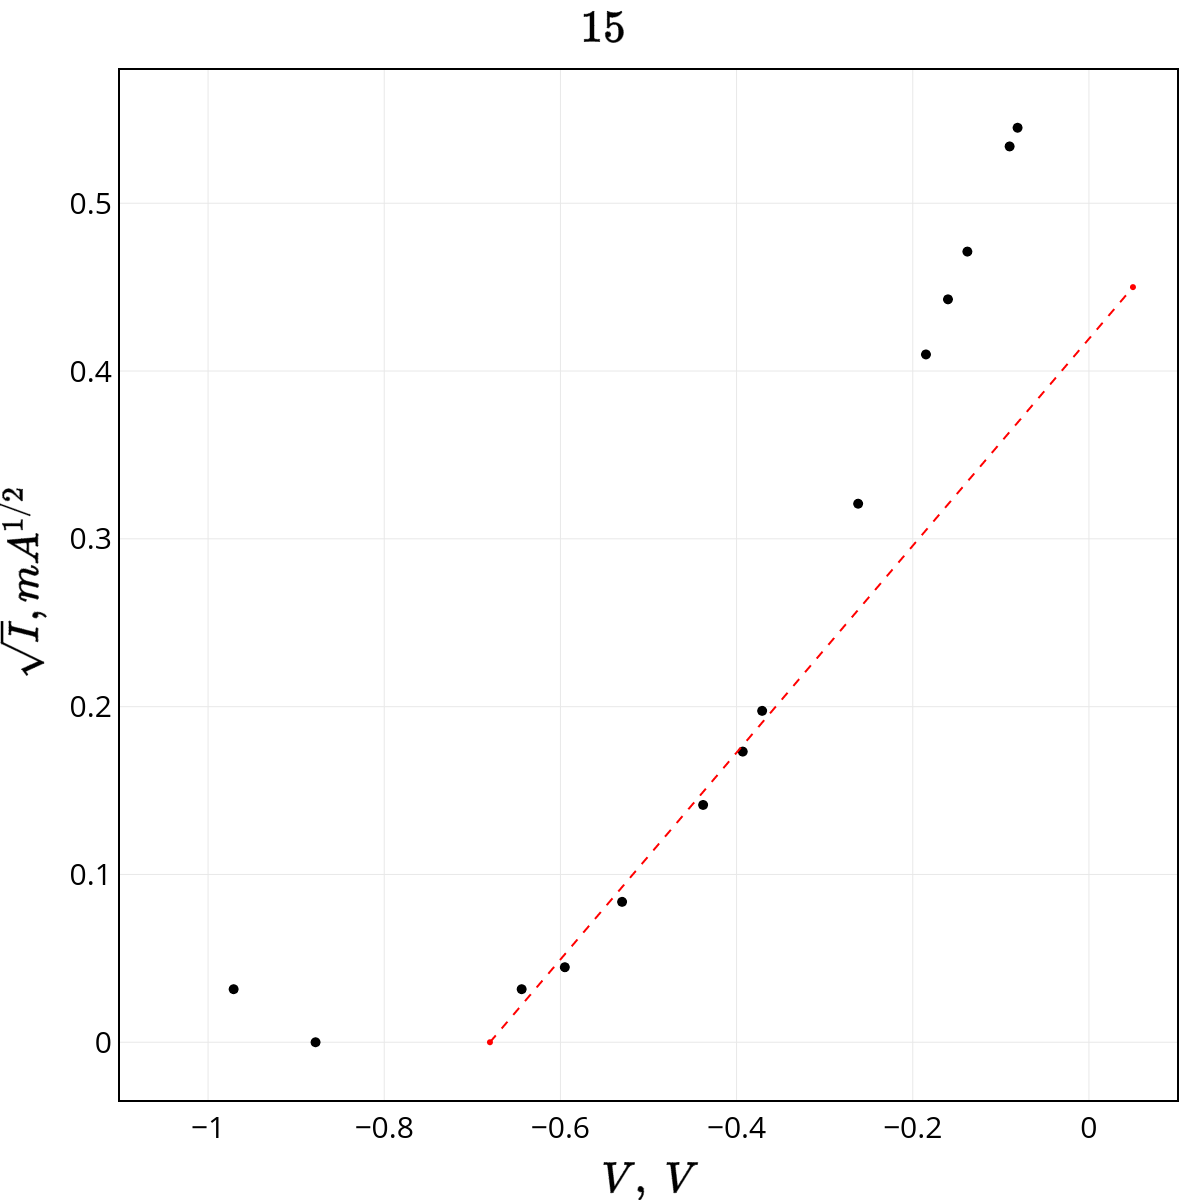
\includegraphics[scale=0.16]{15.png}}
\end{figure}
\begin{figure}
\center{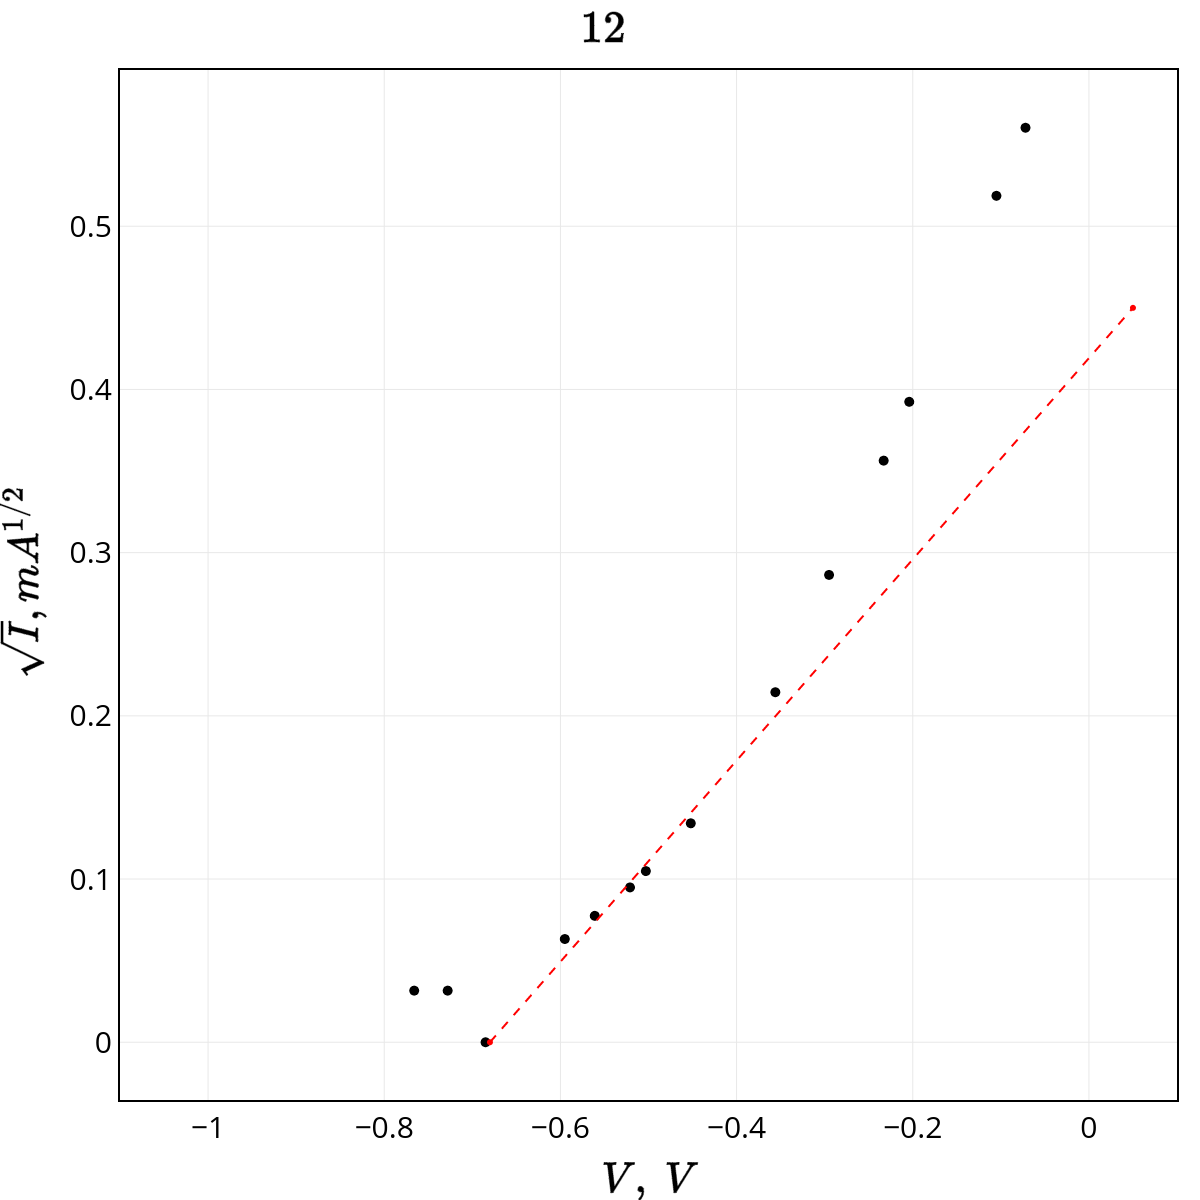
\includegraphics[scale=0.16]{12.png}}
\center{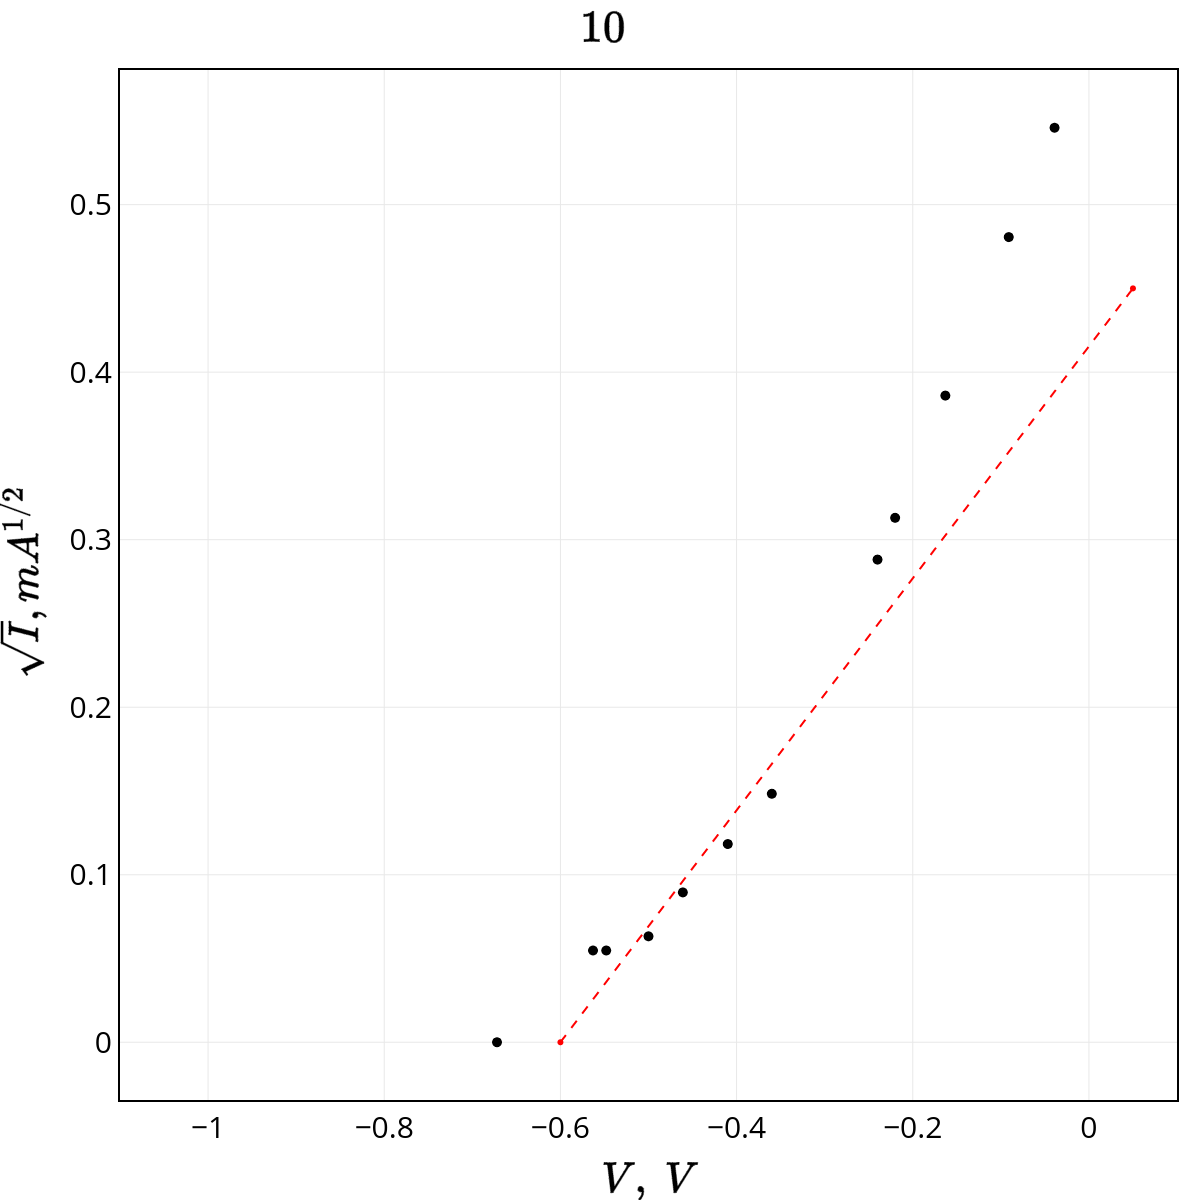
\includegraphics[scale=0.16]{10.png}}
\center{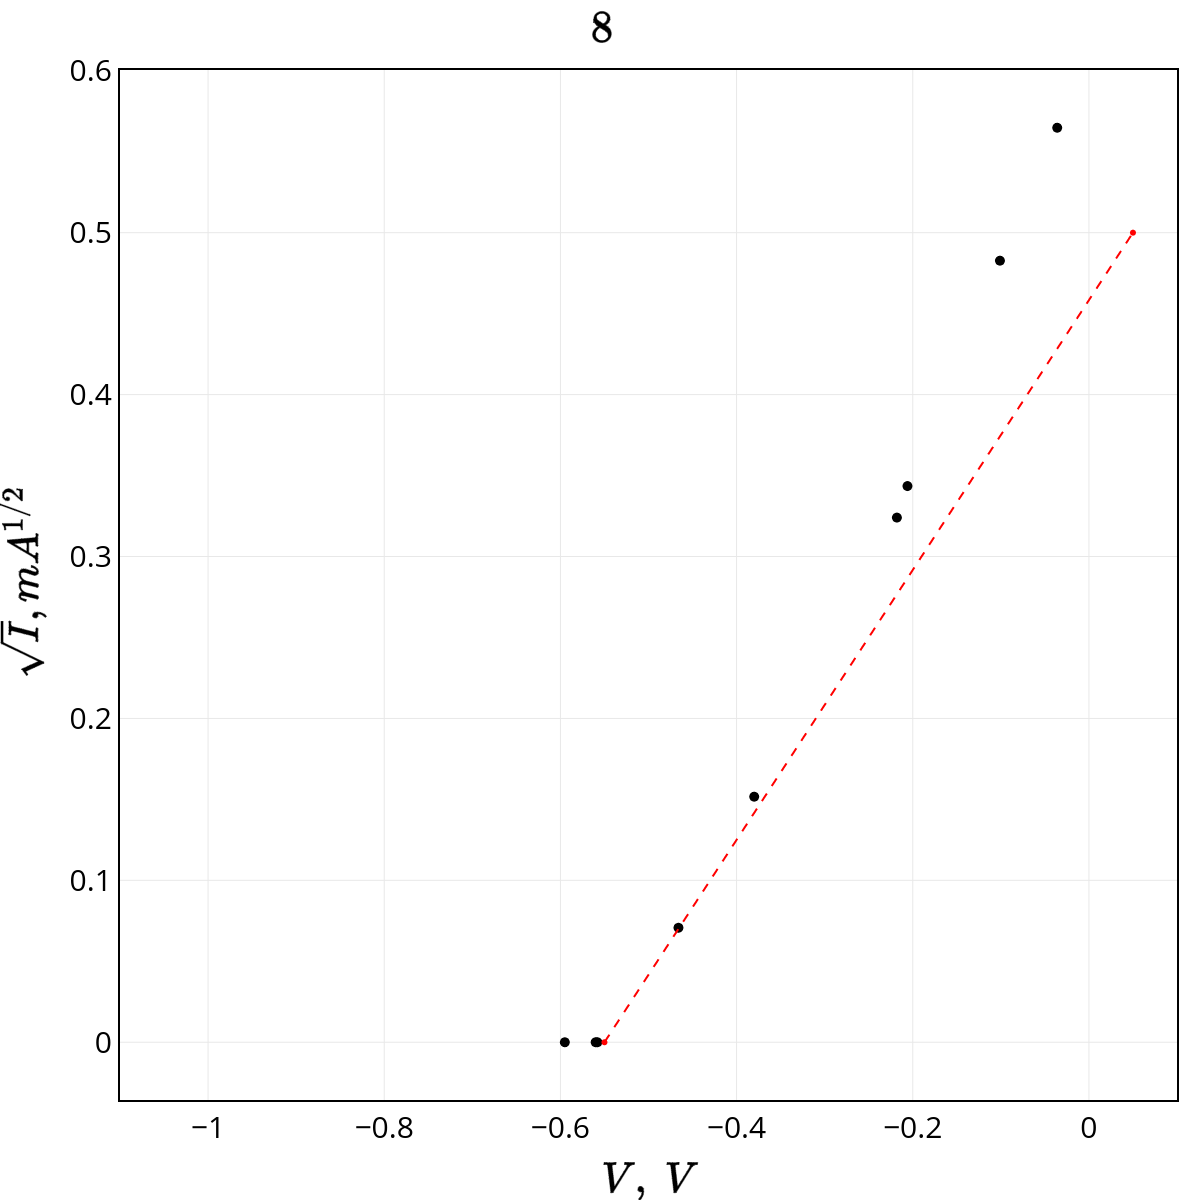
\includegraphics[scale=0.16]{8.png}}
\end{figure}

\begin{figure}[h]
\center{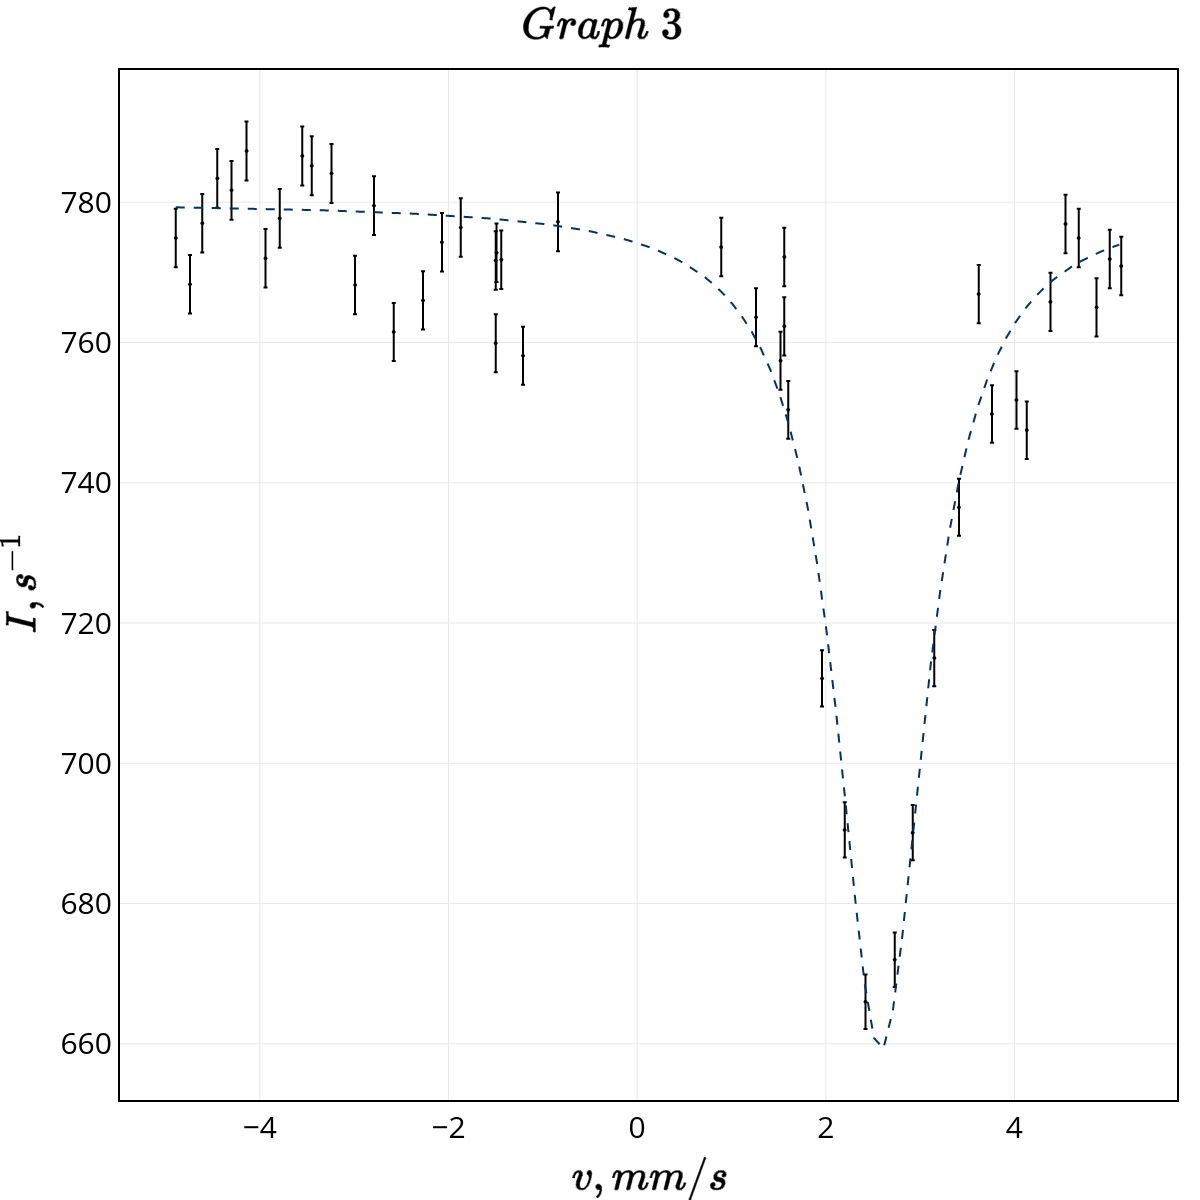
\includegraphics[scale=0.35]{my_plot4.png}}
\end{figure}

\end{enumerate}

\end{document}